\thispagestyle{quantoannone}
\pagestyle{quantoan}
\everymath{\color{quantoan}}
\graphicspath{{../quantoan/pic/}}
\blfootnote{\color{quantoan}\color{quantoan}$^1$Viện Toán học.}
\begingroup
\AddToShipoutPicture*{\put(0,616){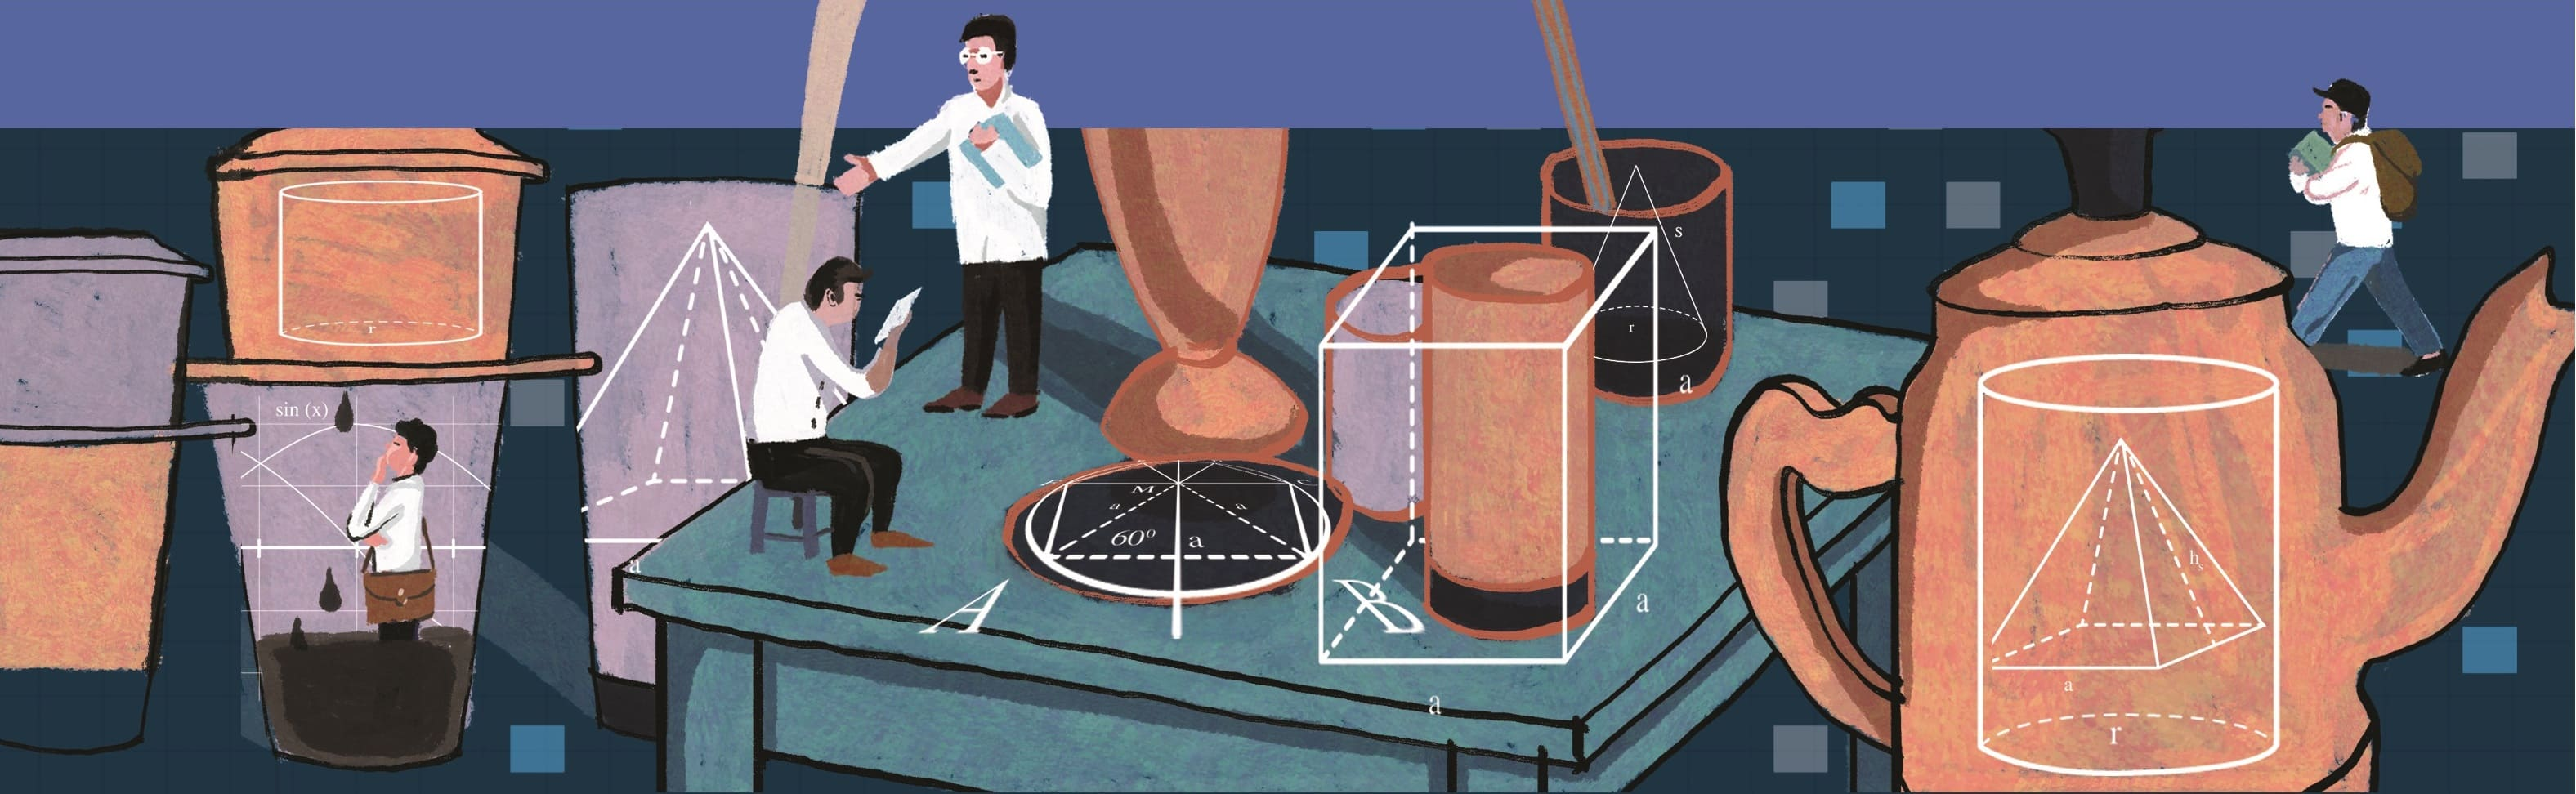
\includegraphics[width=19.3cm]{../bannerquantoan}}}
\AddToShipoutPicture*{\put(156,550){
\includegraphics[scale=1]{../tieude3.pdf}}}
\centering
\endgroup

\vspace*{160pt}

\begin{multicols}{2}	
	Ngày nay số âm đã được học sinh làm quen từ lớp $6$. Nhưng nhân loại đã mất tới $2000$ năm để có thể chấp nhận được nó như cách mà học sinh lớp $6$ ngày nay chấp nhận. 
	\begin{figure}[H]
		\vspace*{-5pt}
		\centering
		\captionsetup{labelformat= empty, justification=centering}
		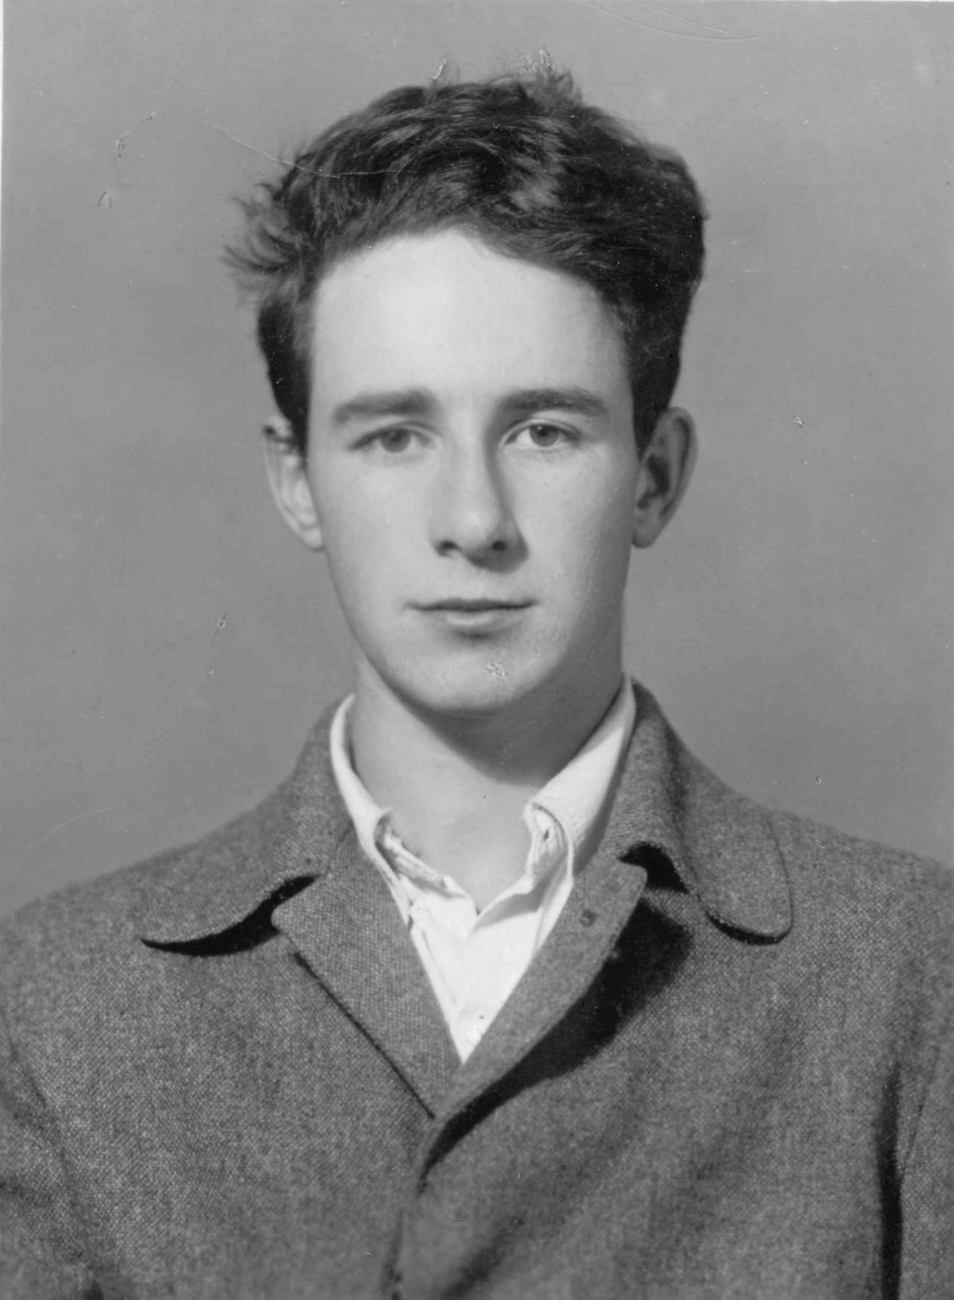
\includegraphics[width= 1\linewidth]{1}
%		\caption{\small\textit{\color{}}}
		\vspace*{-10pt}
	\end{figure}
	Nhìn lại lịch sử cho chúng ta thấy sự vật lộn trong quá trình trừu tượng hóa của Toán học. Hy vọng, theo dõi quá trình vất vả này, các thầy cô giáo THCS sẽ có thêm sự cảm thông đối với những học sinh ``dốt toán". Biết đâu, các em có thể không dốt mà chỉ đang vật lộn với việc phản biện như những nhà toán học kiệt xuất đã từng phản biện về số âm? 
	\vskip 0.1cm
	-- Thế kỷ V TCN, Hy Lạp: Trường phái Pythagoras coi số là ``nhiều đơn vị". Vì vậy với họ ``một" không phải là một số. Không có dấu hiệu nào về số âm trong các ghi chép của họ.
	\vskip 0.1cm
	-- Thế kỷ IV TCN, Hy Lạp: Aristotle đã đưa ra sự phân biệt giữa số (tức là số tự nhiên) và độ lớn (``số đó chia hết thành các số chia mà có thể chia vô hạn"), nhưng không đưa ra dấu hiệu nào về khái niệm số âm hoặc độ lớn âm.
	\vskip 0.1cm
	-- Khoảng năm $300$ TCN, Hy Lạp: Các tập VII, VIII và IX trong cuốn \textit{Cơ sở} của Euclid liên quan đến lý thuyết cơ bản về số. Euclid tiếp tục sự phân biệt của Aristotle giữa số và độ lớn, nhưng vẫn không có dấu hiệu nào về số âm.
	\vskip 0.1cm
	-- Thế kỷ I TCN -- thế kỷ I, Trung Quốc: Trong \textit{Cửu chương Toán thuật}, số âm đã được sử dụng trong chương về giải hệ phương trình. Các que màu đỏ được sử dụng để biểu thị các hệ số dương, màu đen để biểu thị các hệ số âm. Các quy tắc cho số có dấu đã được đưa ra.
	\vskip 0.1cm
	-- Thế kỷ III, Hy Lạp: Dấu hiệu đầu tiên về số âm trong một tác phẩm phương Tây xuất hiện trong cuốn \textit{Số học} của Diophantus, trong đó ông gọi phương trình mà trong ký hiệu hiện đại sẽ được biểu thị bởi $4x + 20 = 0$ là ``vô lý", vì nó sẽ cho nghiệm $x=-5$. Ông cũng nói, ``một số bị trừ, nhân với một số bị trừ, cho một số được cộng (thêm vào)". Vì vậy ông có thể xử lý các biểu thức chẳng hạn như $(x-1)(x-2)$, trong ký hiệu hiện đại. Tuy nhiên, có thể tìm thấy những chỉ dẫn trong tác phẩm của Diophantus rằng ông không có khái niệm trừu tượng về số âm.
	\vskip 0.1cm
	-- Thế kỷ VII, Ấn Độ: Số âm được sử dụng để biểu thị các khoản nợ trong khi số dương biểu thị tài sản. Nhà toán học và thiên văn học Brahmagupta đã sử dụng các số âm để thống nhất phương pháp xử lý phương trình bậc hai của Diophantus từ ba trường hợp thành một trường hợp duy nhất mà chúng ta quen thuộc ngày nay.
	\vskip 0.1cm
	-- Thế kỷ IX, Trung Đông: Mặc dù người Ả Rập đã quen thuộc với các số âm từ công trình của các nhà toán học Ấn Độ, nhưng họ bác bỏ chúng. Cuốn sách \textit{al--Kitāb al--Mukhtaṣar fī Ḥisāb al--Jabr wal--Muqābalah} (mà từ đó chúng ta có thuật ngữ ``algebra" -- đại số) của Muhammad ibn Musa al--Khwarizmi không sử dụng số âm hoặc hệ số âm.
	\vskip 0.1cm
	-- Thế kỷ XIII, Trung Quốc: Các số âm được biểu thị bằng cách vẽ một nét chéo qua chữ số khác không ngoài cùng bên phải của số đó.
	\vskip 0.1cm
	-- Thế kỷ XIII, Châu Âu: Fibonacci không đề cập đến số âm trong cuốn sách \textit{Liber Abaci} của mình, nhưng trong cuốn \textit{Flos} sau đó, ông giải thích nghiệm âm như là sự thua lỗ.
	\vskip 0.1cm
	-- Thế kỷ XV, Châu Âu: Chuquet là người đầu tiên sử dụng số âm trong một tác phẩm ở Châu Âu.
	\vskip 0.1cm
	-- Thế kỷ XVI, Châu Âu: 
	\vskip 0.1cm
	$\circ$ Cardan (Cardano), trong cuốn sách \textit{Ars Magna} của mình đã đưa vào các nghiệm âm của các phương trình và nêu các quy luật cơ bản của hoạt động với các số âm. Ông gọi các số dương là thực và các số âm là hư cấu.
	\vskip 0.1cm
	$\circ$ Viete không thừa nhận số âm.
	\vskip 0.1cm
	-- Thế kỷ XVII, Châu Âu:
	\vskip 0.1cm
	$\circ$ Descartes chấp nhận một phần khái niệm số âm. Ông không công nhận nghiệm âm vì chúng đại diện cho các số ``nhỏ hơn không có gì". Tuy nhiên, ông đã chỉ ra rằng một phương trình có nghiệm âm có thể được biến đổi thành một phương trình có nghiệm dương, điều này khiến ông chấp nhận các số âm.
	\vskip 0.1cm
	$\circ$ Pascal coi phép ``trừ đi $4$ từ $0$" là điều hoàn toàn vô nghĩa.
	\vskip 0.1cm
	$\circ$ Nhà thần học và toán học Antoine Arnauld lập luận chống lại số âm bằng cách sử dụng tỷ lệ; nói rằng tỷ lệ $-1$ trên $1$ giống với tỷ lệ $1$ trên $-1$ là vô lý, vì ``Làm thế nào tỷ lệ giữa một anh nhỏ với một anh lớn hơn lại như giữa anh lớn hơn với anh nhỏ hơn?"
	\vskip 0.1cm
	-- Thế kỷ XVIII, Châu Âu:
	\vskip 0.1cm
	$\circ$ Leibniz đồng ý với lập luận của Arnaud đối với các số âm, nhưng nói rằng vì về hình thức các tỷ lệ như vậy là đúng, nên người ta vẫn có thể tính toán với chúng.
	\vskip 0.1cm
	$\circ$ Maclaurin đã xử lý các đại lượng âm ngang hàng với các đại lượng dương trong tác phẩm \textit{A Treatise of Algebra} của ông.
	\vskip 0.1cm 
	$\circ$ Euler mở đầu tác phẩm \textit{Nhập môn tổng quan về Đại số} với một thảo luận về các phép toán trên các đại lượng dương và âm. Ông sử dụng ví dụ về một khoản nợ để biện minh rằng một số âm lần số dương là một số âm.  
	\vskip 0.1cm
	-- Thế kỷ XIX, Châu Âu: Hamilton đã cố gắng đưa các số âm lên một nền tảng lý thuyết vững chắc (thay vì khái niệm về đại lượng ``nhỏ hơn không có gì") bằng cách sử dụng ý tưởng về ``thời gian thuần túy" xuất phát từ tác phẩm \textit{Phê bình lý tính thuần túy} của Kant. Nỗ lực này có vẻ khá kỳ lạ đối với chúng ta ngày nay, nhưng nó đã giúp ích trong việc phát triển các \textit{quaternion}, ví dụ đầu tiên về một hệ đại số không thỏa mãn tính giao hoán.
	\begin{flushright}
		Theo \url{https://web.ma.utexas.edu/users/mks/326K/Negnos.html}
	\end{flushright}
\end{multicols}